\documentclass{article}
\usepackage{amsmath,amsthm,amsfonts,microtype,amssymb}
\usepackage{enumitem}
\usepackage{parskip}
\usepackage{mathpazo}
\usepackage{tikz-cd}
\usepackage{geometry}
\geometry{top=1in}
\usepackage{float}
\usepackage{graphicx}

\usepackage{hyperref}
\hypersetup{%
  colorlinks=true,
  linkcolor=blue,
  filecolor=blue,
  urlcolor=blue,
  bookmarks=true,
  pdfpagemode=FullScreen,
}


\title{Homework 08 \\ Cellular Homology}
\author{Algebraic Topology - Winter 2021}
\date{Due: \textbf{April 01, 2021, 11:59 pm}}

\begin{document}
\pagenumbering{gobble}
\maketitle

Compute the cellular homology of the following spaces for the coefficients $\mathbb{Q}$, $\mathbb{Z}/p\mathbb{Z}$ (where $p$ is a prime number), and $\mathbb{Z}$ :
\begin{enumerate}
    \item genus $g$ surfaces,
    \item $\mathbb{RP}^2$,
    \item Klein bottle.
    \begin{figure}[H]
        \centering 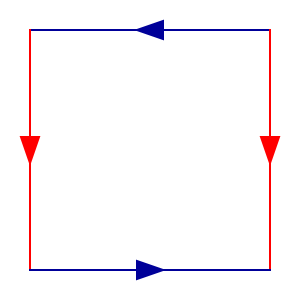
\includegraphics[width=100px]{images/klein-bottle.png}
        \caption{Gluing diagram of a Klein bottle.}
    \end{figure}
\end{enumerate} 


\end{document}
